%─────────────────%
% Header Settings %
%─────────────────%
\def\lecturer{SongHao}
\def\noter{THF}
\def\className{Probability Theory and Mathematical Statistics}
\def\term{III-A}
%─────────────────────%
% Undefined Variables %
%─────────────────────%
\ifx\noter\undefined
    \def\noter{THF}
\else
\fi
\ifx\lecturer\undefined
    \def\lecturer{None}
\else
\fi

%───────────────────%
% Document Settings %
%───────────────────%
\documentclass[12pt,a4paper]{article}

%─────────────────%
% Package Imports %
%─────────────────%
\usepackage[]{amsmath}
\usepackage[]{amssymb}
\usepackage[]{amsthm}
\usepackage[]{array}
\usepackage[]{bm}
\usepackage[]{booktabs}
\usepackage[UTF8]{ctex}
\usepackage[]{fancyhdr}
\usepackage[]{float}
\usepackage[]{geometry}
\usepackage[]{graphicx}
\usepackage[]{hyperref}
\usepackage[]{import}
\usepackage[]{inputenc}
\usepackage[]{mathrsfs}
\usepackage[]{multirow}
\usepackage[]{pdfpages}
\usepackage[]{pgfplots}
\usepackage[]{stmaryrd}
\usepackage[]{tabu}
\usepackage[]{tcolorbox}
\usepackage[]{textcomp}
\usepackage[]{thmtools}
\usepackage[]{tikz}
\usepackage[]{tkz-euclide}
\usepackage[]{url}
\usepackage[]{wrapfig}
\usepackage[dvipsnames]{xcolor}
\usepackage[]{xifthen}
\usepackage[]{yhmath}

%────────────────%
% Fancy Settings %
%────────────────%
\fancypagestyle{CustomStyle}{%
    \fancyhf{}
    \setlength{\headheight}{14.49998pt}
    \fancyhead[R]{\thepage}
    \fancyhead[L]{\lecturer: \className}
}

%──────────────────%
% pgfplot Settings %
%──────────────────%
\usepgfplotslibrary{external}
\pgfarrowsdeclarecombine{twolatex'}{twolatex'}{latex'}{latex'}{latex'}{latex'}
\pgfplotsset{compat=1.12}

%───────────────%
% Tikz Settings %
%───────────────%
\usetikzlibrary{arrows.meta}
\usetikzlibrary{decorations.markings}
\usetikzlibrary{decorations.pathmorphing}
\usetikzlibrary{positioning}
\usetikzlibrary{fadings}
\usetikzlibrary{intersections}
\usetikzlibrary{cd}
\tikzset{->/.style = {decoration={markings,mark=at position 1 with {\arrow[scale=2]{latex'}}},postaction={decorate}}}
\tikzset{<-/.style = {decoration={markings,mark=at position 0 with {\arrowreversed[scale=2]{latex'}}},postaction={decorate}}}
\tikzset{<->/.style = {decoration={markings,mark=at position 0 with {\arrowreversed[scale=2]{latex'}},mark=at position 1 with {\arrow[scale=2]{latex'}}},postaction={decorate}}}
\tikzset{->-/.style = {decoration={markings,mark=at position #1 with {\arrow[scale=2]{latex'}}},postaction={decorate}}}
\tikzset{-<-/.style = {decoration={markings,mark=at position #1 with {\arrowreversed[scale=2]{latex'}}},postaction={decorate}}}
\tikzset{->>/.style = {decoration={markings,mark=at position 1 with {\arrow[scale=2]{latex'}}}postaction={decorate}}}
\tikzset{<<-/.style = {decoration={markings,mark=at position 0 with {\arrowreversed[scale=2]{twolatex'}}},postaction={decorate}}}
\tikzset{<<->>/.style = {decoration={markings,mark=at position 0 with {\arrowreversed[scale=2]{twolatex'}},mark=at position 1 with {\arrow[scale=2]{twolatex'}}},postaction={decorate}}}
\tikzset{->>-/.style = {decoration={markings,mark=at position #1 with {\arrow[scale=2]{twolatex'}}},postaction={decorate}}}
\tikzset{-<<-/.style = {decoration={markings,mark=at position #1 with {\arrowreversed[scale=2]{twolatex'}}},postaction={decorate}}}
\tikzset{circ/.style = {fill, circle, inner sep = 0, minimum size = 3}}
\tikzset{scirc/.style = {fill, circle, inner sep = 0, minimum size = 1.5}}
\tikzset{mstate/.style={circle, draw, blue, text=black, minimum width=0.7cm}}
\tikzset{eqpic/.style={baseline={([yshift=-.5ex]current bounding box.center)}}}
\tikzset{commutative diagrams/.cd,cdmap/.style={/tikz/column 1/.append style={anchor=base east},/tikz/column 2/.append style={anchor=base west},row sep=tiny}}

%──────────────────────%
% Theorem Environments %
%──────────────────────%
\theoremstyle{definition}
\declaretheoremstyle[
    headfont=\bfseries\sffamily\color{ForestGreen!70!black}, bodyfont=\normalfont,
    mdframed={
        linewidth=2pt,
        rightline=false, topline=false, bottomline=false,
        linecolor=ForestGreen, backgroundcolor=ForestGreen!5,
    }
]{thmgreenbox}
\declaretheoremstyle[
    headfont=\bfseries\sffamily\color{NavyBlue!70!black}, bodyfont=\normalfont,
    mdframed={
        linewidth=2pt,
        rightline=false, topline=false, bottomline=false,
        linecolor=NavyBlue, backgroundcolor=NavyBlue!5,
    }
]{thmbluebox}
\declaretheoremstyle[
    headfont=\bfseries\sffamily\color{NavyBlue!70!black}, bodyfont=\normalfont,
    mdframed={
        linewidth=2pt,
        rightline=false, topline=false, bottomline=false,
        linecolor=NavyBlue
    }
]{thmblueline}
\declaretheoremstyle[
    headfont=\bfseries\sffamily\color{RawSienna!70!black}, bodyfont=\normalfont,
    mdframed={
        linewidth=2pt,
        rightline=false, topline=false, bottomline=false,
        linecolor=RawSienna, backgroundcolor=RawSienna!5,
    }
]{thmredbox}
\declaretheoremstyle[
    headfont=\bfseries\sffamily\color{RawSienna!70!black}, bodyfont=\normalfont,
    numbered=no,
    mdframed={
        linewidth=2pt,
        rightline=false, topline=false, bottomline=false,
        linecolor=RawSienna, backgroundcolor=RawSienna!1,
    },
    qed=\qedsymbol
]{thmproofbox}
\declaretheoremstyle[
    headfont=\bfseries\sffamily\color{NavyBlue!70!black}, bodyfont=\normalfont,
    numbered=no,
    mdframed={
        linewidth=2pt,
        rightline=false, topline=false, bottomline=false,
        linecolor=NavyBlue, backgroundcolor=NavyBlue!1,
    },
]{thmexplanationbox}
\declaretheorem[style=thmblueline,numbered=no,name=Notation]{notation}
\declaretheorem[style=thmgreenbox,numbered=no,name=Definition]{defi}
\declaretheorem[style=thmproofbox,numbered=no,name=Proof]{replacementproof}
\newtheorem*{aim}{Aim}
\newtheorem*{assumption}{Assumption}
\newtheorem*{axiom}{Axiom}
\newtheorem*{claim}{Claim}
\newtheorem*{conjecture}{Conjecture}
\newtheorem*{cor}{Corollary}
\newtheorem*{eg}{Example}
\newtheorem*{exercise}{Exercise}
\newtheorem*{ex}{Exercise}
\newtheorem*{fact}{Fact}
\newtheorem*{law}{Law}
\newtheorem*{lemma}{Lemma}
\newtheorem*{prop}{Proposition}
\newtheorem*{question}{Question}
\newtheorem*{remark}{Remark}
\newtheorem*{rrule}{Rule}
\newtheorem*{thm}{Theorem}
\newtheorem*{warning}{Warning}
% \newtheorem{ncor}[nthm]{Corollary}
% \newtheorem{nlemma}[nthm]{Lemma}
% \newtheorem{nprop}[nthm]{Proposition}
% \newtheorem{nthm}{Theorem}[section]
\renewenvironment{proof}[1][\proofname]{\vspace{-10pt}\begin{replacementproof}}{\end{replacementproof}}

%─────────────%
% Math Symbol %
%─────────────%

%────────────%
% Beginnings %
%────────────%
\title{\textbf{Part III-B: \className}}
\author{Lecture by \lecturer\\Note by \noter}
\pagestyle{CustomStyle}
%────────────────────────────────%
% Page Settings (set when print) %
%────────────────────────────────%
% \addtolength{\parskip}{-1mm}
% \addtolength{\parindent}{-2mm}
% \geometry{left=0.5cm,right=0.5cm,top=0.5cm,bottom=0.5cm}


%──────────%
% Document %
%──────────%
\begin{document}
\maketitle
\tableofcontents
\section{排列组合}%
\label{sub:排列组合}
1. 加法原理:完成事件有多类方案

2. 乘法原理:完成事件分多步

\begin{eg}
    有三种馒头,四种米饭

    加法原理:只吃一种,共$7$种

    乘法原理:先吃馒头,后吃米饭,共$12$种
\end{eg}
\subsection{排列}%
\label{sub:排列}
1. 不重复排列

从$n$ 个不同元素中取出$m$个排列,不放回
\[
    P_n^m=n\left( n-1 \right) \left( n-2 \right) \ldots\left( n-m+1 \right)=\frac{n!}{\left( n-m \right) !} 
.\] 
\begin{eg}
    $P^5_{10}=10\times 9\times 8\times 7\times 6$
\end{eg}

2. 全排列

\[
    P^n_n=n!
.\] 
\begin{eg}
    $P_{0}^{0}=0! =1$
\end{eg}

3. 重复排列

从$n$ 个不同元素中取出$m$个排列,可放回
\[
    (P_n^m)=n^m
.\] 

\subsection{组合}%
\label{sub:组合}

从 $n$ 个不同元素中取出$m$ 个,不排列
\[
    C_n^m=\frac{P_n^m}{m!}=\frac{n!}{\left( n-m \right)! m!}
.\] 
\[
    \begin{cases}
        C_{n}^{m}=C_{n}^{n-m}\\
        C_{n}^{n}=C_{n}^{0}=1
    \end{cases}
.\] 

\begin{eg}
    在书架上有序放置五本书,求其顺序为$1,2,3,4,5$ 的概率:

    总样本点个数:$P_{5}^{5}$

    目标事件样本点个数:$2$(顺序、逆序)

    概率: \[
        P=\frac{2}{P_{5}^{5}}= \frac{1}{60}
    .\] 
\end{eg}
\begin{eg}
    有四个邮箱,两封信,求:

    1. 前两个邮箱各有一封的概率

    总样本点个数:$4\times 4=16$ 

    第一个邮箱有一封信且第二个邮箱有一封信的样本点个数:$P_{2}^{2}=2$ (第一封信前往$1,2$ ,第二封信前往$2,1$)

    概率:\[
        P=\frac{2}{16}=\frac{1}{8}
    .\] 

    2. 第二个邮箱恰有一封信的概率

    事件:从两封信中抽一封放到邮箱$2$ 中,剩余的$1$ 封信在除$2$以外的三个邮箱中选一个放入

    即:\[
        C_{2}^{1}C_{3}^{1}=6
    .\] 

    概率:\[
        P=\frac{C_{2}^{1}C_{3}^{1}}{4\times 4}=\frac{3}{8}
    .\] 

    3. 两封信不在一个邮箱内的概率

    事件:一封信随机投入一个邮箱,另一封信投入剩余的三个邮箱

    概率:
    \[
        P=\frac{4\times 3}{4\times 4}=\frac{3}{4}
    .\] 
    
    或:$1-$ 信在同一个邮箱的概率

    $\displaystyle{=1-\frac{4}{16}=\frac{3}{4}}$
\end{eg}
\begin{eg}
    有$5$ 白$4$ 黑共$9$ 个球,任取$3$ 个球,求:

    1. 取出$2$ 白$1$ 黑的概率:\[
        P=\frac{C_{5}^{2}C_{4}^{1}}{C_{9}^{3}}
    .\] 

    2. 全是白球的概率:\[
        P=\frac{C_{5}^{3}}{C_{9}^{3}}
    .\] 

    3. 颜色相同的概率:\[
        P=\frac{C_{5}^{3}+C_{4}^{3}}{C_{9}^{3}}
    .\] 

    4. 颜色不同的概率:\[
        P=\frac{C_{5}^{1}C_{3}^{2}}{C_{9}^{3}}+\frac{C_{5}^{2}C_{3}^{1}}{C_{9}^{3}}
    .\] 
\end{eg}
\begin{eg}
    有$a$ 个白球,$b$ 个黑球

    1. 任取一个是白球的概率:
    \[
        P=\frac{a}{a+b}
    .\] 

    2. 接连取出$m$ 个球$\left( m\in \left[ 1,a+b \right]  \right) $ ,第$m$ 个是白球的概率:\\
    法1: 将所有球排为一排,为全排列:$\left( a+b \right) !$ 
    
    要使第$m$ 个球是白球:

    先任从白球中拿一个放入该位置,其他的球全排列
    \[
        P=\frac{a\left( a+b-1 \right) !}{\left( a+b \right) !}=\frac{a}{a+b}
    .\] 
    法2:只取$m$ 个球

    从$a+b$ 个中取出$m$ 个并排好:$P_{a+b}^{m}$

    要使第$m$ 个是白球,单独挑一个白球放在第$m$ 个上

    然后在剩余的球中取出$m-1$个并排好: $P_{a+b-1}^{m-1}$ 

    概率:
    \[
        P=\frac{P_{a+b-1}^{m-1}\times a}{P_{a+b}^{m}}=\frac{a\times \frac{\left( a+b-1 \right) !}{\left( a+b-1-\left( m-1 \right)  \right) !}}{\frac{\left( a+b \right) !}{\left( a+b-m \right) !}}=\frac{a}{a+b}
    .\] 
    法3. 先取第$m$ 个位置的球

    一共有$a+b$个球,选$a$个白球中的一个放入即可:
    \[
        P=\frac{a}{a+b}
    .\] 
\end{eg}
\section{事件的概率}%
\label{sec:事件的概率}

\subsection{概率的基本描述}%
\label{sub:概率的基本描述}
发生$A$事件的可能性大小称作概率,记作$P\left( A \right) $.
\begin{eg}
   抛一枚硬币,正面朝上的概率为:$P\left( A \right) =P\left( \bar{A} \right) = 0.5$
\end{eg}
性质:

1. $P\left( \Omega \right) =1$ 

2. $P\left( \varnothing \right) =0$ 

3. $P\left( A \right) \in [0,1]$

\subsection{古典概率模型}%
\label{sub:古典概率模型}
古典概率模型应满足两个条件:

1. 样本空间中存在有限个样本

2. 所有样本点出现的可能性相同(等可能性)
\begin{eg}
    扔硬币,观察朝上的面

    该事件对应的样本空间只有两个样本:正面朝上与反面朝上

    正面朝上与反面朝上的可能性相同:$P\left( A \right) =P\left( B \right) =0.5$ 

    因此为古典概率模型。
\end{eg}
古典概率模型的概率计算:
\[
    P\left( A \right) =\frac{N\left( A \right) }{N\left( \Omega \right) }= \frac{\omega\left( A \right) }{\omega\left( \Omega \right) }
.\] 
\begin{notation}
    $N\left( A \right) $ :$A$事件所包含的基本事件个数

    $\omega\left( A \right)$:$A$事件所包含的样本点个数
\end{notation}
\begin{notation}
    古典概率模型的特性:

    1. 非负性:$P\left( A \right) \in \left[ 0,1 \right] $
    
    2. 规范性:$P\left( \Omega \right) =1,P\left( \varnothing \right) =0$

    3. 有限可加性:$A_1,A_2\ldots A_n$互不相容,则:\[
        P\left( \sum_{i=1}^{n} A_i \right) =\sum_{i=1}^{n} P\left( A_i \right) 
    .\] 
    缺点:

    1. 有限个结果

    2. 等可能性
\end{notation}
\subsection{几何概率模型}%
\label{sub: 几何概率模型}
\begin{eg}
    有一长方形,右边部分的阴影占面积的$\frac{1}{2}$,扔一个质子,落在阴影的概率为$\frac{1}{2}$.
\end{eg}
\begin{center}
    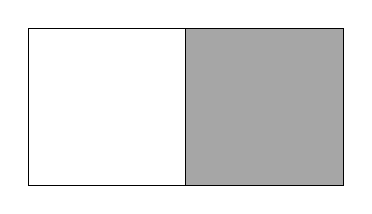
\begin{tikzpicture}
        \filldraw [gray,opacity=0.7] (0,1) rectangle (2,-1);
        \draw [] (-2,1) rectangle (2,-1);
        \draw [] (0,1)--(0,-1);
    \end{tikzpicture}
\end{center}
\begin{eg}
     一条线段长$3$ ,阴影部分占$\left[ 1,2 \right] $ ,扔一个质子,落在阴影的概率为$\frac{1}{3}$.
\end{eg}
\begin{center}
    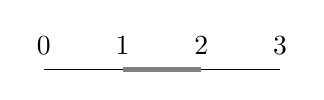
\begin{tikzpicture}
        \node [] (0) at (0,0.3) {$0$};
        \draw [] (0,0)--(1,0) node at(1,0.3) {$1$};
        \draw [line width=2,gray] (1,0)--(2,0) node [black] at(2,0.3) {$2$};
        \draw [] (2,0)--(3,0) node at(3,0.3) {$3$};
    \end{tikzpicture}
\end{center}
与几何概率模型有关的元素:

1. 线段

2. 平面

3. 立体

\[
    P\left( A \right) =\frac{\mu\left( G \right) }{\mu\left( \Omega \right) }
.\] 
$\mu\left( G \right) $ :度量
\begin{eg}
    会面问题:

    甲乙两人约定从六点到七点见面,先到的人等$15$ 分钟,且这一小时内甲乙可在任意时刻到达,求甲乙见面的概率。
\end{eg}
\begin{figure}[ht]
    \centering
    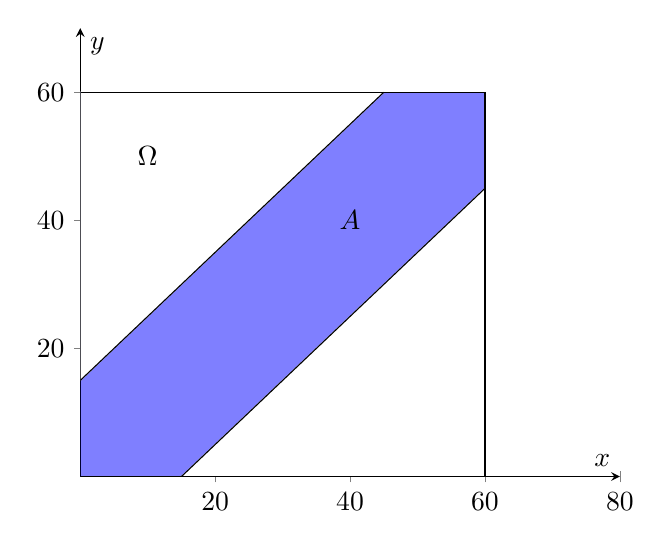
\begin{tikzpicture}
        \begin{axis}[
            xlabel=$x$,ylabel=$y$,
            xmin=0, xmax=80,
            ymin=0, ymax=70,
            axis lines=middle,
        ]
            \filldraw [blue,opacity=0.5] (0,60) rectangle (60,0);
            \filldraw [white] (0,15)--(0,60)--(45,60)--cycle (15,0)--(60,0)--(60,45)--cycle;
            \draw [] (0,60) rectangle (60,0);
            \node [] (Omega) at(10,50) {$\Omega$};
            \node [] (A) at(40,40) {$A$};
            \addplot[domain=0:45]{x+15};
            \addplot[domain=0:60]{x-15};
        \end{axis}
    \end{tikzpicture}
\end{figure}
    令$A$ 为事件两人见面,$x$ 为甲到达的时间,$y$ 为乙到达的时间,$A$ 发生的情况如下:

    1. 甲先到,乙后到,即:\[
        y>x,y-x \le 15
    .\] 

    2. 乙先到,甲后到,即:
    \[
        y<x,x-y \le 15
    .\] 

    即:
    \[
        \left| y-x \right| \le 15
    .\] 

    如图:
\[
    S_A=60\times 60-45\times 45\times \frac{1}{2}\times 2=1575
.\] 
\[
    S_{\Omega}=60\times 60=3600
.\] 
\[
    P\left( A \right) =\frac{S_A}{S_{\Omega}}=\frac{1575}{3600}=\frac{7}{16}
.\] 
\begin{eg}
    蒲丰投针问题:\\
    有两条平行线,距离为$d$ ,朝平面内投掷长度为$l\left( l<d \right) $ 的针,求针与任意一个平行线相交的概率

    假设$x$ 表示针的中点离最近的一根线的距离,有:
    \[
        x\in \left[ 0,\frac{d}{2} \right] 
    .\]

    即针的一部分可以出来,但针的中点不能出来。

    假设$\varphi$ 是针与线的夹角,有:
    \[
        \varphi\in \left[ 0,\pi \right] 
    .\] 

    因此该事件全集写为:\[
        \Omega=\left\{ \left( \varphi,x \right) |\varphi\in \left[ 0,\pi \right] ,x\in \left[ 0,\frac{d}{2} \right]  \right\} 
    .\] 
    \begin{center}
        \begin{tikzpicture}
            \draw [line width=1] (-6,2)--(6,2);
            \draw [line width=1] (-6,-2)--(6,-2);
            \draw [] (-4,1)--(-5.5,0.4);
            \filldraw [] (-4.75,0.7) circle (2pt);
            \draw [] (-4.75,0.7)--(-4.75,2);
            \node [] (x) at(-4.5,1.5) {$x$};
            \node [] (l) at (-4.75,0.2) {$l$};
            \draw [] (5,2)--(5,-2);
            \node [] (d) at (4.75,0) {$d$};
            \draw [dashed] (-4,1)--(-1.5,2);
            \draw [] (-2,2) arc (180:200:0.5) node at(-2.5,1.8) {$\varphi$ };
        \end{tikzpicture}
    \end{center}
    \begin{notation}
        针的左右位置并不体现,但上下位置用$x$ 体现出来。
    \end{notation}

    在坐标轴中绘制出全集图像:
    \begin{figure}[htbp]
        \centering
        \begin{tikzpicture}
            \begin{axis}[
                trig format plots=rad,
                xlabel=$x$,
                xmin=0,
                xmax=3,
                xtick distance=1,
                xticklabels={0,,$\frac{d}{4}$,$\frac{d}{2}$,$\frac{3d}{4}$},
                ylabel= $\varphi$,
                ymin=0,
                ymax=pi*3/2,
                ytick distance=pi/2,
                yticklabels={0,,$\frac{\pi}{2}$,$\pi$,$\frac{3\pi}{2}$},
                axis lines=middle,
            ]
                \draw [] (0,pi)--(2,pi)--(2,0);
                \node [] (Omega) at (1,pi/2) {$\Omega$}; 
            \end{axis}
        \end{tikzpicture}
    \end{figure}

    判断相交条件:
    \begin{center}
        \begin{tikzpicture}
            \draw [line width=1] (-6,2)--(6,2);
            \draw [line width=1] (-6,-2)--(6,-2);
            \draw [] (-4,2.2)--(-5.5,1.6);
            \filldraw [] (-4.75,1.9) circle (2pt);
            \draw [] (-4.75,1.9)--(-4.75,2);
            \draw [] (5,2)--(5,-2);
            \node [] (d) at (4.75,0) {$d$};
            \draw [] (-5.7,2.5) rectangle (-3.7,1.3);
            
        \end{tikzpicture}
    \end{center}

    放大观察:
    \begin{center}
        \begin{tikzpicture}
            \draw [] (-6.5,0)--(0,2.6);
            \filldraw [] (-3.25,1.3) circle (2pt);
            \draw [] (-6,2)--(0,2);
            \draw [dashed] (-3.25,1.3)--(-3.25,2);
            \filldraw [red] (-1.5,2) circle (2pt) (-3.25,2) circle (2pt);
            \draw [] (-2,2) arc (180:200:0.5);
            \node [] (varphi) at (-2.5,1.8) {$\varphi$};
            \node [] (x) at (-3.6,1.6) {$x$};
            \node [] (A) at (-3.25,1) {$A$};
            \node [] (B) at (-3.25,2.3) {$B$};
            \node [] (C) at (-1.5,1.6) {$C$};
            \node [] (displaystylefracl2) at (-4.5,0) {$\displaystyle{\frac{l}{2}}$};
            
        \end{tikzpicture}
    \end{center}    

    可得相交的条件:\[
        AC\le \frac{l}{2}
    .\]

    即:\[
        \frac{x}{\sin\left( \varphi \right) }\le \frac{l}{2}
    .\] 

    即:
    \[
        x\le \frac{l}{2}\cdot \sin\left( \varphi \right) 
    .\] 

    即事件发生可写做:
    \[
        A=\left\{ \left( \varphi,x \right) |\varphi\in \left[ 0,\pi \right] ,x\in \left[ 0,\frac{l}{2}\cdot \sin\left( \varphi \right) \right]   \right\} 
    .\] 
    
    在坐标轴上绘制该区域:
    \begin{center}
        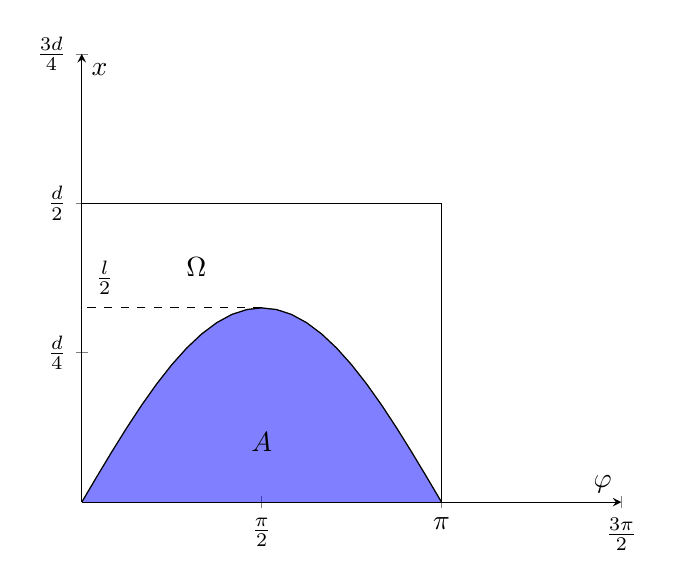
\begin{tikzpicture}
            \begin{axis}[
                trig format plots=rad,
                ylabel=$x$,
                ymin=0,
                ymax=3,
                ytick distance=1,
                yticklabels={0,,$\frac{d}{4}$,$\frac{d}{2}$,$\frac{3d}{4}$},
                xlabel= $\varphi$,
                xmin=0,
                xmax=pi*3/2,
                xtick distance=pi/2,
                xticklabels={0,,$\frac{\pi}{2}$,$\pi$,$\frac{3\pi}{2}$},
                axis lines=middle,
            ]
                \draw [fill=blue,opacity=0.5,domain=0:3.14]plot(\x,{1.3*sin(\x r)});
                \draw [] (0,2)--(pi,2)--(pi,0);
                \node [] (Omega) at (1,pi/2) {$\Omega$}; 
                \addplot [domain=0:pi] {1.3*sin(x)};
                \draw [dashed] (pi/2,1.3)--(0,1.3);
                \node [] (fracl2) at (0.2,1.5) {$\frac{l}{2}$};
                \node [] (A) at (pi/2,0.4) {$A$};
            \end{axis}
        \end{tikzpicture}
    \end{center}

    即有:\[
        P=\frac{S_A}{S_\Omega}
    .\] 

    使用定积分求$S_A$:
     \[
        S_A=\int_{0}^{\pi} \frac{l}{2}\sin\left( \varphi \right)  \mathrm{d}\varphi=l
    .\]
    \[
        S_\Omega=\frac{d}{2}\cdot \pi
    .\] 
    \[
        P=\frac{l}{\frac{d}{2}\cdot \pi}=\frac{2l}{\pi d}
    .\] 
\end{eg}
\begin{remark}
    蒙特卡洛方法:
    
    实际实验时,使用了$N$ 根针,有$n$ 根落在线上,频率为\[
        P_0=\frac{n}{N}
    .\] 

    由蒙特卡洛方法有$P_0\approx P$,即:
    \[
        \frac{2l}{\pi d}\approx \frac{n}{N}
    .\]
    \[
        \pi \approx \frac{2lN}{nd}
    .\]     
    
    即:通过蒙特卡洛方法,设定一个未知数,通过计算得知包含该未知数的概率,实验得到频率,可以计算出该未知数的近似值。
\end{remark}
\begin{notation}
    几何概率模型特性:
    
    完全可加性($A_i$ 彼此互不相容):\[
        P\left( \bigcup_{i=1}^{\infty}A_i \right) =\sum_{i=1}^{\infty} P\left( A_i \right) 
    .\] 
\end{notation}
\section{频率与概率}%
\label{sec:频率与概率}
频率:看一个事件是否发生,做$n $次实验,发生了$m$ 次,记为:
\[
    \omega_n\left( A \right) =\frac{m}{n}
.\] 
\begin{eg}
    扔硬币$100$ 次,正面朝上$54$ 次

    频率:\[
        \omega_{100}=\frac{54}{100}=0.54
    .\] 

    概率:\[
        P=\frac{1}{2}=0.5
    .\] 
\end{eg}
\begin{notation}
    频率特性:

    1. 非负性:\[
        \omega_n\left( A \right) \in \left[ 0,1 \right] 
    .\]
    
    2. 规范性:必然事件的频率等于$1$ ,不可能事件频率等于$0$ ,即:
    \[
        \omega_n\left( \Omega \right) =1,\omega_n\left( \varnothing \right) =0
    .\]

    3. 可加性:若$A_1,A_2,\ldots,A_m$互不相容,则:\[
        \omega_n\left( \bigcup_{i=1}^{m}A_i \right) =\sum_{i=1}^{m} \omega_n\left( A_i \right) 
    .\] 
\end{notation}
\begin{notation}
    随着实验次数增多,频率会逐渐接近于一个值

    这个值称作统计概率

    如扔硬币正面朝上的频率会接近于$0.5$
\end{notation}

\section{公理化}%
\label{sec:公理化}

提到了四种定义:

1. 描述

2. 古典

3. 几何

4. 统计

这些定义均含有三个性质:

1. 非负性

2. 规范性

3. 可加性

公理化尝试提出公理,找到其中相同的部分并将其统一
\subsection{公理}%
\label{sub:公理}
\begin{axiom}
    非负性:
    \[
        P\left( A \right) \in \left[ 0,1 \right] 
    .\] 
\end{axiom}

\begin{axiom}
    规范性:
    \[
        P\left( \Omega \right) =1
    .\]
\end{axiom}

\begin{axiom}
    可加性:

    $A_1,A_2,\ldots$互不相容,则:
    \[
        P\left( \bigcup_{i=1}^{\infty}A_i \right) =\sum_{i=1}^{\infty} P\left( A_i \right)
    .\] 
\end{axiom}

\subsection{性质}%
\label{sub:性质}
\begin{rrule}
    $P\left( \varnothing \right) =0$
\end{rrule}
\begin{proof}
    \[
        \Omega=\Omega+\varnothing+\varnothing+\ldots
    .\] 
    \[
        P\left( \Omega \right) =P\left( \Omega+\varnothing+\varnothing+\ldots \right) 
    .\] 
    由于$\Omega$与$\varnothing$ 互不相容,所以由无穷可加性:
    \[
        P\left( \Omega \right) =P\left( \Omega \right) +P\left( \varnothing \right) +P\left( \varnothing \right) +\ldots
    .\] 
    \[
        P\left( \varnothing \right) +P\left( \varnothing \right) +\ldots=0
    .\] 
    由非负性:$P\left( \varnothing \right) \in \left[ 0,1 \right] $ ,即:$P\left( \varnothing \right) =0$
\end{proof}

\begin{rrule}
    有限可加性:$A_1,A_2,\ldots,A_n$ 互不相容,则:\[
        P\left( \bigcup_{i=1}^{n}A_i \right) =\sum_{i=1}^{n} P\left( A_i \right) 
    .\] 
\end{rrule}
\begin{proof}
    有$A_1,A_2,\ldots,A_n$ 互不相容,再接上无穷多个$\varnothing$ 也互不相容

    由完全可加性可得:
    \begin{equation}
        \begin{aligned}
            &P\left( A_1+A_2+\ldots+A_n+\varnothing+\varnothing+\ldots \right)\\
            &= P\left( A_1 \right) +P\left( A_2 \right) +\ldots+P\left( A_n \right) +P\left( \varnothing \right) +P\left( \varnothing \right) +\ldots\\
            &= P\left( A_1 \right) +P\left( A_2 \right) +\ldots+P\left( A_n \right) \\
        \end{aligned}
    \end{equation}
    即:$P\left( A_1+A_2+\ldots+A_n \right)=P\left( A_1 \right) +P\left( A_2 \right) +\ldots+P\left( A_n \right) $
\end{proof}

\begin{rrule}
    $P\left( \overline{A} \right) =1-P\left( A \right) $
\end{rrule}
\begin{proof}
    $A$ 和$\overline{A}$ 不相容,且$A+\overline{A}=\Omega$ ,则:
    \[
        P\left( \Omega \right) =P\left( A+\overline{A} \right) =P\left( A \right) +P\left( \overline{A} \right) =1
    .\] 
    即:$P\left( \overline{A} \right) =1-P\left( A \right) $ 
\end{proof}
\begin{cor}
    $A_1,A_2,\ldots,A_n$ 为完备事件组,利用有限可加性:
    \[
        P\left( \Omega \right) =P\left( \bigcup_{i=1}^{n}A_i \right) =P\left( A_1 \right) +P\left( A_2 \right) +\ldots+P\left( A_n \right) =1
    .\] 
\end{cor}
\begin{rrule}
    $P\left( A-B \right) =P\left( A \right) -P\left( AB \right) $
\end{rrule}
\begin{proof}
    令$A =\left( A-B \right) \cup AB$

    由于$A-B$ 和$AB$ 互不相容,由有限可加性:
     \[
        P\left( A \right) =P\left( \left( A-B \right) \cup AB \right) =P\left( A-B \right) +P\left( AB \right) 
    .\] 
    即$P\left( A-B \right) =P\left( A \right) -P\left( AB \right) $
\end{proof}
\begin{rrule}
    \[
        P\left( A-B \right) =P\left( A \right) -P\left( B \right)
    \]

    and
    \[
        P\left( A \right) \ge P\left( B \right) 
    \] 
    
    if
    \[
        B\subset A
    .\] 

\end{rrule}
\begin{proof}
   由$B\subset A$ 可得:\[
       P\left( AB \right) =P\left( B \right) 
   .\] 

   即$P\left( A-B \right) =P\left( A \right) -P\left( B \right) $ 

   由非负性:\[
       P\left( A-B \right) =P\left( A \right) -P\left( B \right) \ge 0
   .\] 
   
   即:$P\left( A \right) \ge P\left( B \right) $
\end{proof}
\begin{rrule}
    加法公式(very important)

    对$\forall A,B$ 有:\[
        P\left( A+B \right) =P\left( A \right) +P\left( B \right) -P\left( AB \right) 
    .\] 
\end{rrule}
\begin{proof}
    画图如下:
    \begin{center}
        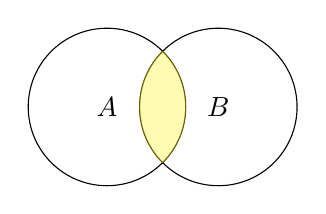
\begin{tikzpicture}
            \draw [] ({-1/sqrt(2)},0) circle [radius=1] node at({-1/sqrt(2)},0) {$A$};
            \draw [] ({1/sqrt(2)},0) circle [radius=1] node at({1/sqrt(2)},0) {$B$};
            \filldraw [yellow,opacity=0.3] (0,{1/sqrt(2)}) arc (135:225:1) (0,{-1/sqrt(2)}) arc (-45:45:1);
        \end{tikzpicture}
    \end{center}
    $P\left( A \right) +P\left( B \right) $ 会多加一次$P\left( AB \right) $ (图中黄色部分),因此减去即可。
\end{proof}
\begin{notation}
    $A,B$ 不相容时该公式也成立:$P\left( AB \right) =P\left( \varnothing \right) =0$ 

    即有限可加性:$P\left( A+B \right) =P\left( A \right) +P\left( B \right) $
\end{notation}
\begin{eg}
    三个事件相加:\[
        P\left( A+B+C \right)  
    \] 
    \[
        =P\left( A \right) +P\left( B \right) +P\left( C \right) -P\left( AB \right) -P\left( BC \right) -P\left( AC \right) +P\left( ABC \right)
    .\] 
\end{eg}
\begin{proof}
    画图如下,图示部分为$P\left( ABC \right) $ :
    \begin{center}
        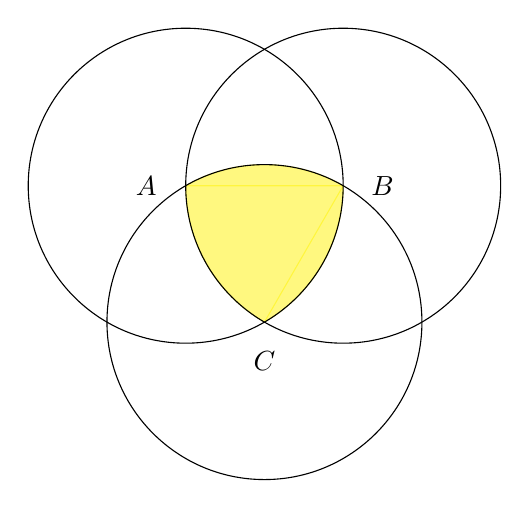
\begin{tikzpicture}
            \filldraw [yellow,opacity=0.5] (-1,0) arc (180:240:2) (1,0) arc (60:120:2) (0,{-sqrt(3)}) arc (-60:0:2) (-1,0)--(1,0)--(0,{-sqrt(3)});
            \draw [] (-1,0) circle [radius=2] node at(-1.5,0) {$A$};
            \draw [] (1,0) circle [radius=2] node at(1.5,0) {$B$};
            \draw [] (0,{-sqrt(3)}) circle [radius=2] node at(0,{-sqrt(3)-0.5}) {$C$};
        \end{tikzpicture}
    \end{center}
    当$P\left( A \right) +P\left( B \right) +P\left(  C\right) $时,图示部分被重复累加了$3$ 次,减去$P\left( AB \right) +P\left( BC \right) +P\left( AC \right) $ 后图示部分被减去了$3$ 次,因此加上$P\left( ABC \right) $ 即可。
\end{proof}



\subsection{例题}%
\label{sub:例题}
\begin{eg}
    $P\left( A \right) =0.4,P\left( B \right) =0.3,P\left( A+B \right)=0.6 $,求$P\left( A\bar{B} \right) $ 

    画图如下:
    \begin{center}
        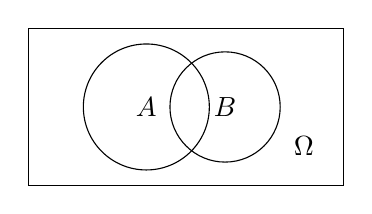
\begin{tikzpicture}
            \draw [] (-2,1) rectangle (2,-1) node at(1.5,-0.5) {$\Omega$};
            \draw [] (-0.5,0) circle [radius=0.8] node at(-0.5,0) {$A$};
            \draw [] (0.5,0) circle [radius=0.7] node at(0.5,0) {$B$};
        \end{tikzpicture}
    \end{center}
    
    即$P\left( AB \right) =0.1$,$P\left( A\bar{B} \right) = P\left( A \right) -P\left( AB \right) =0.3$

    或:$P\left( A+B \right) =P\left( A \right) +P\left( B \right) -P\left( AB \right) $ 

    即:$P\left( AB \right) =P\left( A+B \right) -P\left( A \right) -P\left( B \right) =0.1$ 

    后续同上。
\end{eg}
\begin{eg}
    \[
        P\left( A \right) =P\left( B \right) =P\left( C \right) =\frac{1}{4}
    .\] 且\[
        P\left( AB \right) =0,P\left( AC \right) =P\left( BC \right) =\frac{1}{16}
    .\] 求$A,B,C$至少一个发生的概率和 $A,B,C$都不发生的概率
    
    $P\left( A+B+C \right) $

    $=P\left( A \right) +P\left( B \right) +P\left( C \right) -P\left( AB \right) -P\left( AC \right) -P\left( BC \right) +P\left( ABC \right)$

    $\displaystyle{=\frac{3}{4}-0-\frac{1}{16}*2+P\left( ABC \right) }$
     
    由于$P\left( ABC \right) \in P\left( AB \right) $ 

    所以:$P\left( ABC \right) \le P\left( AB \right) =0$,即:$P\left( ABC \right) =0$ 

    即:\[
        P\left( A+B+C \right) =\frac{5}{8}
    .\] 

    求$P\left( \bar{A}\bar{B}\bar{C} \right) $ :正难则反原则,可先求出$A,B,C$ 至少发生一个的概率,由于两个事件互斥,即有:$P\left( A+B+C \right) +P\left( \bar{A}\bar{B}\bar{C} \right) =1$

    即:\[
        P\left( \bar{A}\bar{B}\bar{C} \right) =\frac{3}{8}
    .\] 

\end{eg}

\begin{notation}
    不可能事件的概率为$0$ ,但反之,概率为$0$ 的事件不一定是不可能事件

    即:概率为$0$ 的事件可能会发生
    \begin{eg}
        朝一条长为$1$ ,头尾分别是$0,1$ 的线上扔一个质子,扔到一个点$A$ 的概率为$0$ ,但该事件可能发生
    \end{eg}
\end{notation}

\begin{eg}
    有四个白球,三个黑球,任取三个球,求这三个球至少有两个白球的概率

    所有的情况:从七个中取三个

    目标:从四个白球中取两个/三个,从三个黑球中取一个/不取

    即:\[
        P\left( A \right) =\frac{C_{4}^{2}C_{3}^{1}+C_{4}^{3}}{C_{7}^{3}}
    .\] 
\end{eg}
\begin{eg}
    一个人看管两台机床,第一台机床无需看管的概率为$0.9$ ,第二台为$0.8$ ,两台都需要看管的概率为$0.02$ ,求一小时内至少一台需要看管的概率

    画图即可:
    \begin{center}
        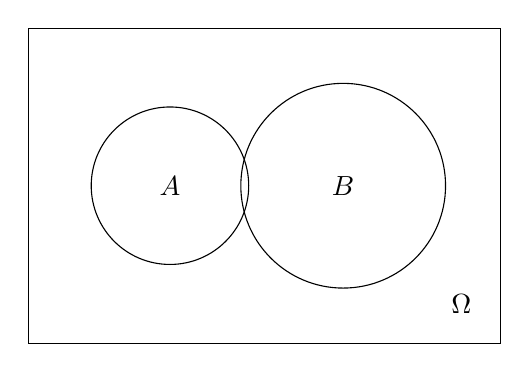
\begin{tikzpicture}
            \draw [] (-3,2) rectangle (3,-2) node at(2.5,-1.5) {$\Omega$};
            \draw [] (-1.2,0) circle [radius=1] node at(-1.2,0) {$A$};
            \draw [] (1,0) circle [radius=1.3] node at(1,0) {$B$};
            
        \end{tikzpicture}
    \end{center}
    \[
        P\left( A \right) =0.1,P\left( B \right) =0.2,P\left( AB \right) =0.02
    .\] 
    
    易得要求的是$P\left( A+B \right) =P\left( A \right) +P\left( B \right) -P\left( AB \right) =0.28$
\end{eg}
\begin{eg}
    一共有$20$ 个产品,一等、二等、三等个数分别为:$6,10,4$ ,从中取出$3$ 个,求至少两件等级相同的概率

    正难则反原则:求所有等级都不相同的概率

    所有情况:$20\to 3$

    目标:$6\to 1,10\to 1,4\to 1$ 

    概率:
     \[
        P\left( \bar{A} \right) =\frac{C_{6}^{1}C_{10}^{1}C_{4}^{1}}{C_{20}^{3}}
    .\] 
     \[
        P\left( A \right) =1-P\left( \bar{A} \right) =\frac{15}{19}
    .\] 

\end{eg}
\begin{eg}
    生日问题:一个班上有$n$ 个学生,求至少两个人生日相同的概率

    正难则反:求所有人生日不同的概率

    所有情况:$365^n$ 

    目标:$365\cdot 364\cdot 363\cdot \ldots\cdot (365-\left( n-1 \right)) $ 

    概率:\[
        P\left( A \right) =1-\frac{365\cdot 364\cdot \ldots\cdot (365-\left( n-1 \right)) }{365^{n}}
    .\]

    当$n=55$时,$P\left( A \right) \approx 0.99$

    即这个班上几乎必然有生日在同一天的人
\end{eg}

\end{document}

